\documentclass{article}
\usepackage[paperwidth=222mm,paperheight=120mm,margin=4mm,noheadfoot]{geometry}
\usepackage{amsmath,amssymb}
\usepackage{helvet}
\usepackage{tikz}
\renewcommand{\familydefault}{\sfdefault}
\usetikzlibrary{arrows.meta,backgrounds,calc,fit,positioning}

% Okabe--Ito palette: colour-blind safe and separable in grayscale.
\definecolor{oiBlue}{HTML}{0072B2}
\definecolor{oiSky}{HTML}{56B4E9}
\definecolor{oiOrange}{HTML}{E69F00}
\definecolor{oiGreen}{HTML}{009E73}
\definecolor{ink}{HTML}{263238}
\definecolor{muted}{HTML}{607D8B}
\definecolor{hair}{HTML}{B0BEC5}
\definecolor{panel}{HTML}{F7F9FA}
\definecolor{bluefill}{HTML}{EDF6FB}
\definecolor{orangefill}{HTML}{FFF7E8}
\definecolor{greenfill}{HTML}{EAF6F1}

\tikzset{
  every node/.style={text=ink},
  module/.style={draw=hair, fill=white, rounded corners=1.4pt,
    line width=.55pt, align=center, inner xsep=4.2pt, inner ysep=3.2pt,
    font=\fontsize{8.6}{9.6}\selectfont},
  numerical/.style={module, draw=oiBlue, fill=bluefill, line width=.75pt},
  llm/.style={module, draw=oiOrange, fill=orangefill, dashed, line width=.8pt},
  simulator/.style={module, draw=oiGreen, fill=greenfill, line width=.9pt},
  state/.style={module, draw=muted, fill=white, line width=.75pt},
  flow/.style={-{Latex[length=2.1mm,width=1.25mm]}, draw=ink, line width=.68pt},
  feedback/.style={-{Latex[length=2.1mm,width=1.25mm]}, draw=oiBlue, line width=.78pt},
  guide/.style={-{Latex[length=2.1mm,width=1.25mm]}, draw=oiOrange,
    dashed, line width=.85pt},
  tinylabel/.style={font=\fontsize{7.2}{8.0}\selectfont, text=muted,
    align=center, fill=white, inner sep=1.1pt},
  paneltitle/.style={font=\fontsize{9.4}{10.4}\selectfont\bfseries,
    text=ink, anchor=west},
  panelsub/.style={font=\fontsize{7.4}{8.2}\selectfont, text=muted,
    anchor=west},
  panelbox/.style={draw=hair, fill=panel, rounded corners=2pt,
    line width=.55pt, inner sep=5pt}
}

\begin{document}
\thispagestyle{empty}
\noindent
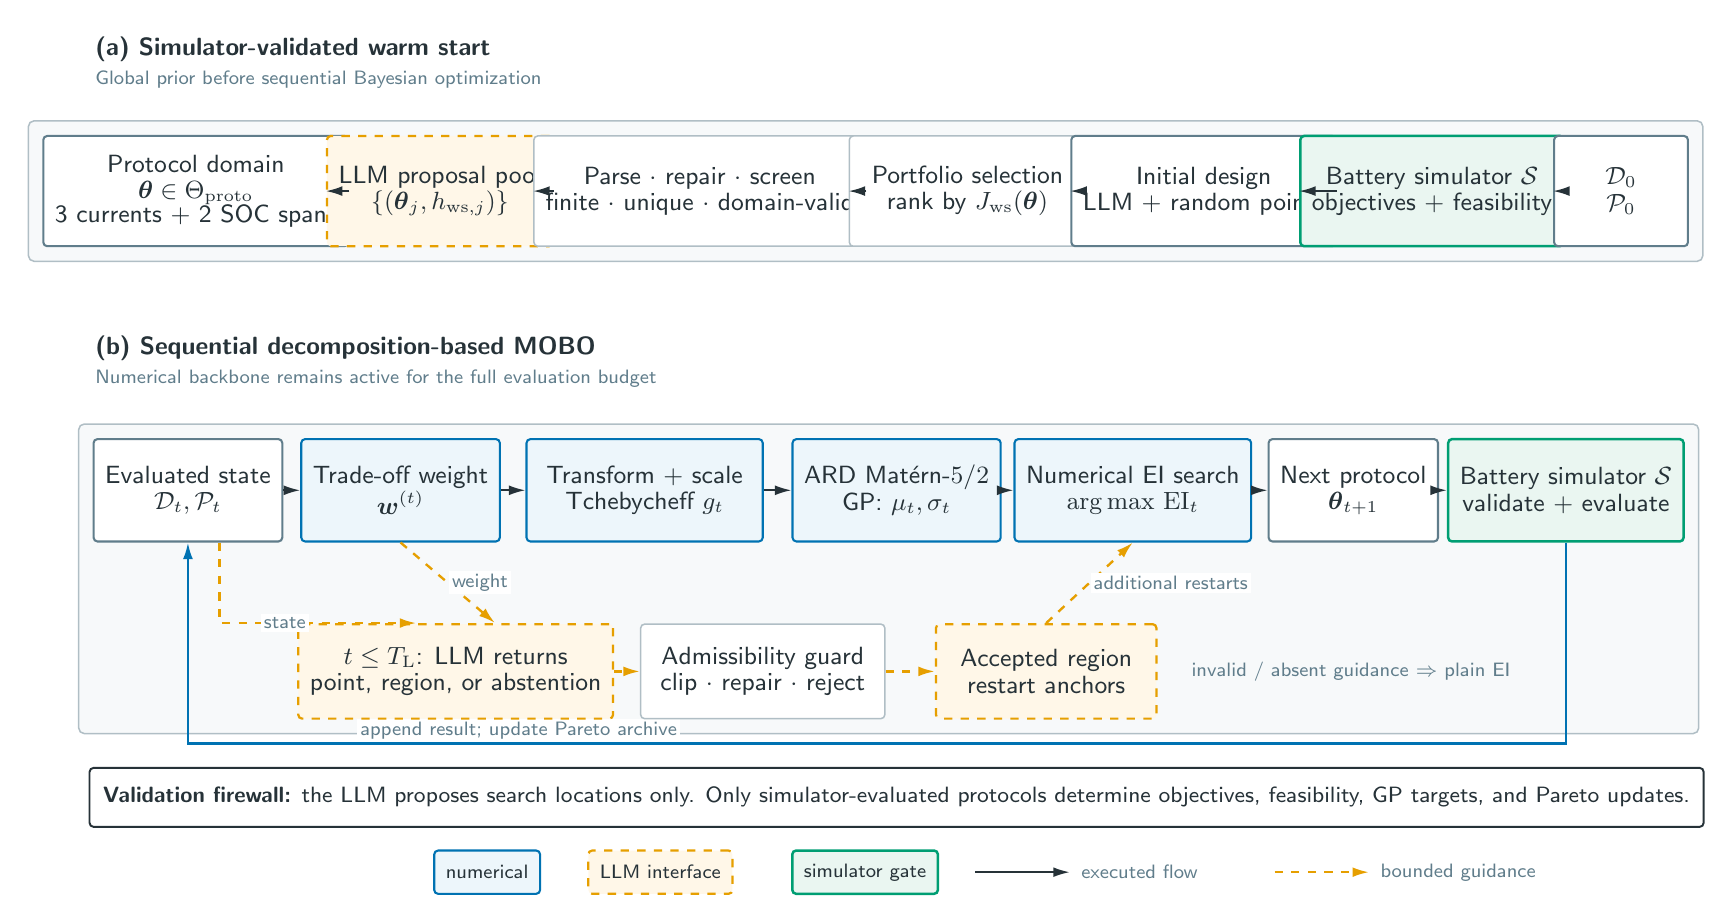
\begin{tikzpicture}[x=1mm,y=1mm]

% ---------------------------------------------------------------------------
% Panel A: the global, simulator-validated warm start.
% ---------------------------------------------------------------------------
\node[paneltitle] at (0,84) {(a) Simulator-validated warm start};
\node[panelsub] at (0,80.2) {Global prior before sequential Bayesian optimization};

\node[state, minimum width=25mm, minimum height=14mm] (domain) at (14,66)
  {Protocol domain\\$\boldsymbol\theta\in\Theta_{\mathrm{proto}}$\\[-1pt]
   3 currents + 2 SOC spans};

\node[llm, minimum width=28mm, minimum height=14mm] (pool) at (45,66)
  {LLM proposal pool\\$\{(\boldsymbol\theta_j,h_{\mathrm{ws},j})\}$};

\node[module, minimum width=30mm, minimum height=14mm] (screen) at (78,66)
  {Parse $\cdot$ repair $\cdot$ screen\\
   finite $\cdot$ unique $\cdot$ domain-valid};

\node[module, minimum width=30mm, minimum height=14mm] (portfolio) at (112,66)
  {Portfolio selection\\rank by $J_{\mathrm{ws}}(\boldsymbol\theta)$};

\node[state, minimum width=24mm, minimum height=14mm] (mix) at (142,66)
  {Initial design\\LLM + random points};

\node[simulator, minimum width=25mm, minimum height=14mm] (sim0) at (171,66)
  {Battery simulator $\mathcal S$\\objectives + feasibility};

\node[state, minimum width=17mm, minimum height=14mm] (db0) at (195,66)
  {$\mathcal D_0$\\$\mathcal P_0$};

\draw[flow] (domain) -- (pool);
\draw[flow] (pool) -- (screen);
\draw[flow] (screen) -- (portfolio);
\draw[flow] (portfolio) -- (mix);
\draw[flow] (mix) -- (sim0);
\draw[flow] (sim0) -- (db0);

\begin{scope}[on background layer]
  \node[panelbox, fit=(domain)(pool)(screen)(portfolio)(mix)(sim0)(db0)] (panelA) {};
\end{scope}

% ---------------------------------------------------------------------------
% Panel B: numerical MOBO loop with a strictly bounded LLM side branch.
% ---------------------------------------------------------------------------
\node[paneltitle] at (0,46) {(b) Sequential decomposition-based MOBO};
\node[panelsub] at (0,42.2) {Numerical backbone remains active for the full evaluation budget};

\node[state, minimum width=20mm, minimum height=13mm] (dbt) at (13,28)
  {Evaluated state\\$\mathcal D_t,\mathcal P_t$};

\node[numerical, minimum width=22mm, minimum height=13mm] (weight) at (40,28)
  {Trade-off weight\\$\boldsymbol w^{(t)}$};

\node[numerical, minimum width=30mm, minimum height=13mm] (scalar) at (71,28)
  {Transform + scale\\Tchebycheff $g_t$};

\node[numerical, minimum width=25mm, minimum height=13mm] (gp) at (103,28)
  {ARD Mat\'ern-$5/2$\\GP: $\mu_t,\sigma_t$};

\node[numerical, minimum width=27mm, minimum height=13mm] (ei) at (133,28)
  {Numerical EI search\\$\arg\max\,\mathrm{EI}_t$};

\node[state, minimum width=21mm, minimum height=13mm] (next) at (161,28)
  {Next protocol\\$\boldsymbol\theta_{t+1}$};

\node[simulator, minimum width=24mm, minimum height=13mm] (simt) at (188,28)
  {Battery simulator $\mathcal S$\\validate + evaluate};

\draw[flow] (dbt) -- (weight);
\draw[flow] (weight) -- (scalar);
\draw[flow] (scalar) -- (gp);
\draw[flow] (gp) -- (ei);
\draw[flow] (ei) -- (next);
\draw[flow] (next) -- (simt);
\draw[feedback] (simt.south) -- ++(0,-25.5) -|
  node[tinylabel,pos=.38,above]{append result; update Pareto archive} (dbt.south);

% Bounded early-window guidance: dashed outline/edges redundantly encode LLM use.
\node[llm, minimum width=34mm, minimum height=12mm] (region) at (47,5)
  {$t\leq T_{\mathrm L}$: LLM returns\\point, region, or abstention};

\node[module, minimum width=31mm, minimum height=12mm] (guard) at (86,5)
  {Admissibility guard\\clip $\cdot$ repair $\cdot$ reject};

\node[llm, minimum width=28mm, minimum height=12mm] (anchors) at (122,5)
  {Accepted region\\restart anchors};

\draw[guide] ([xshift=4mm]dbt.south) |- node[tinylabel,pos=.73,left]{state}
  ([xshift=-5mm]region.north);
\draw[guide] (weight.south) -- node[tinylabel,right]{weight}
  ([xshift=5mm]region.north);
\draw[guide] (region) -- (guard);
\draw[guide] (guard) -- (anchors);
\draw[guide] (anchors.north) -- node[tinylabel,right]{additional restarts} (ei.south);
\node[tinylabel, anchor=west, fill=none, text=muted] at (140,5)
  {invalid / absent guidance $\Rightarrow$ plain EI};

\begin{scope}[on background layer]
  \node[panelbox, fit=(dbt)(weight)(scalar)(gp)(ei)(next)(simt)(region)(guard)(anchors)] (panelB) {};
\end{scope}

% Bottom safety rule: the conceptual invariant of the method.
\node[draw=ink, fill=white, rounded corners=1.5pt, line width=.7pt,
  minimum width=205mm, minimum height=7.5mm,
  font=\fontsize{8.1}{9.0}\selectfont, align=center] at (103,-11)
  {\textbf{Validation firewall:} the LLM proposes search locations only. Only simulator-evaluated protocols determine objectives, feasibility, GP targets, and Pareto updates.};

% Compact visual key.
\node[numerical, minimum width=13mm, minimum height=5.5mm,
  font=\fontsize{7.0}{7.8}\selectfont] at (51,-20.5) {numerical};
\node[llm, minimum width=13mm, minimum height=5.5mm,
  font=\fontsize{7.0}{7.8}\selectfont] at (73,-20.5) {LLM interface};
\node[simulator, minimum width=13mm, minimum height=5.5mm,
  font=\fontsize{7.0}{7.8}\selectfont] at (99,-20.5) {simulator gate};
\draw[flow] (113,-20.5) -- (125,-20.5);
\node[tinylabel, anchor=west, fill=none] at (126,-20.5) {executed flow};
\draw[guide] (151,-20.5) -- (163,-20.5);
\node[tinylabel, anchor=west, fill=none] at (164,-20.5) {bounded guidance};

\end{tikzpicture}
\end{document}
